\documentclass[11pt]{amsart}
\usepackage[margin=2.5cm]{geometry}           % See geometry.pdf to learn the layout options. There are lots.
\geometry{letterpaper} % ... or a4paper or a5paper  or letterpaper ... 
%\geometry{landscape}                % Activate for for rotated page geometry
%\usepackage[parfill]{parskip}    % Activate to begin paragraphs with an empty line rather than an
%indent
\usepackage{graphicx}
\usepackage{amssymb}
\usepackage{epstopdf}
\usepackage{amsmath}
\usepackage{comment}
\DeclareGraphicsRule{.tif}{png}{.png}{`convert #1 `dirname #1`/`basename #1 .tif`.png}

\title{Applying the Henyey method to tidally induced stellar oscillations}
\author{Andrew Bunting}
%\date{}                                           % Activate to display a given date or no date
%
\begin{document}

\maketitle

\section{Introduction}

This is an explanation, record and walkthrough of the derivation and origin of the equations used in the code to solve the stellar oscillation equations using the Henyey method.  Initially the discussion will be fairly abstract and general, but this will become more and more specific as we go along.

To start with, we will address the structure of the method overall, to get a feel for the big picture to try to avoid getting bogged down in details.  Then we will move through the relevant sections of the method in sequence, first with the recurrence relations for $\underline{\alpha}$ and $\vec{\gamma}$; we will then discuss the application of the outer boundary conditions; after that we will discuss the recurrence relation for $\vec{u}$ and $\vec{v}$; finishing off with a discussion of practicalities, such as minimising the amount of memory needed.


\section{Overall structure}

To start with, the structure of the equations must be set out.  This method is used to solve four linear, first order differential equations.  Whilst it is not necessary in general, here we will be restricting ourselves to the case where the two pairs of variables are on a staggered grid, with $\vec{u}$ being evaluated at the outer edge of the cell, and $\vec{v}$ being evaluated at the centre of the cell, where $\vec{u} = \left( a, b \right)^{T}$ and $\vec{v} = \left( c, d \right)^{T}$

The boundary equations are split, two apply at the centre ($\vec{u} = 0$) and two apply at the surface of the star.  Because of this, it is difficult to work with a solution from one boundary to the other, as the problem is under-constrained until all boundary conditions can be applied.

In order to get around this, the Henyey method uses a two-stage approach.  A relation between $\vec{u}$ and $\vec{v}$ is used, which is formulated in such a way that conditions upon the coefficients can be found which reproduce the central boundary condition.  This relation is

\begin{equation} \label{eq:relation}
\vec{u}_{k}  + \underline{\alpha}_{k}  \vec{v}_{k}  + \vec{\gamma}_{k}  = 0,
\end{equation}
\\
which obeys the central boundary condition if $\underline{\alpha}_{0} = 0$ and $\vec{\gamma}_{0} = 0$ are used as a surrogate.  Recurrence relations for the coefficients in this equation ($\underline{\alpha}$ and $\vec{\gamma}$) are used to calculate the values of these coefficients at each point, including at the surface.  Using the surface boundary conditions with the outermost coefficients, the values for $\vec{u}$ and $\vec{v}$ can be evaluated.  Then, another recurrence relation can be found, which relates the values of $\underline{\alpha}$, $\vec{\gamma}$, $\vec{u}$ and $\vec{v}$ at a given point, to the values of $\vec{u}$ and $\vec{v}$ at the adjacent point just inside.  This enables them to be evaluated at all points throughout the star, and the solution is complete.

To describe this problem more specifically, we must look at the structure of the equations in question, and the variables involved.  Two equations involve the derivative of $\vec{u}$ but not $\vec{v}$, and the other two include the derivative of $\vec{v}$ but not $\vec{u}$.  Because of this, we can split the four equations into two matrix equations:

\begin{equation} \label{eq:ACD}
\underline{A}_{k,k+1} \vec{u}_{k} + \underline{C}_{k,k+1} \vec{u}_{k+1} + \underline{D}_{k,k+1} \vec{v}_{k+1} = \vec{M}_{k,k+1},
\end{equation} 

\begin{equation} \label{eq:EFH}
\underline{E}_{k,k+1} \vec{u}_{k} + \underline{F}_{k,k+1} \vec{v}_{k} + \underline{H}_{k,k+1} \vec{v}_{k+1} = \vec{N}_{k,k+1}.
\end{equation} 
\\

This structure means that the two equations with derivatives of $\vec{u}$ make up equation \ref{eq:ACD}, which is evaluated at the midpoint of cell $k+1$; and the two equations with derivatives of $\vec{v}$ make up equation \ref{eq:EFH}, which is evaluated at the outer edge of cell k.  Notably, this structure ensures that the matrices B and G, which would be included in a more general formulation, are ignored from the start, as they would be null at all points, which helps to avoid issues like trying to invert a singular matrix.  In this discussion, the star is divided into $J$ cells, so $k$ will run from $0$ to $J-1$. 


\begin{figure}
\begin{center}
\label{fig:overview}
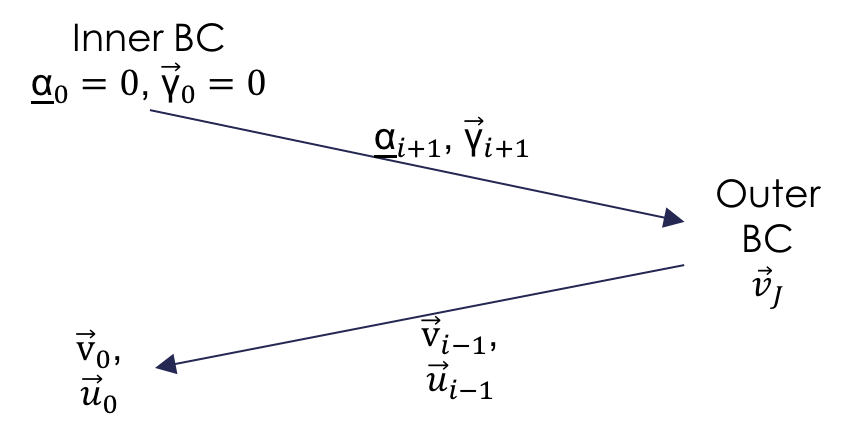
\includegraphics[width = 0.5 \textwidth]{Overview.png}
\caption{A diagrammatic overview of the Henyey method, showing what is being evaluated at each stage of the code.}
\end{center}
\end{figure}







\section{$\underline{\alpha}$ and $\vec{\gamma}$ recurrence relations}

The relation $\vec{u} + \underline{\alpha} \vec{v} + \vec{\gamma} = 0$ is formulated this way as it enables the central boundary condition to be re-expressed as $\underline{\alpha} = 0$ and $\vec{\gamma} = 0$ at the centre.  By combining this initial condition with a recurrence relation, we can iterate outwards to find their values at all points in the star.

There are many different ways to formulate the recurrence relation, which will all be mathematically equivalent, although the particular form of the relations may have some computational effects, depending on how they are implemented.  The relevant equations are equations \ref{eq:relation}, \ref{eq:ACD} and \ref{eq:EFH}.  The key idea is to use these equations to reflect the structure of equation \ref{eq:relation}, evaluated at $k+1$, and to compare coefficients in order to get the equations for $\underline{\alpha}_{k+1}$ and $\vec{\gamma}_{k+1}$.

For ease of reading, the subscripts on the coefficients in equations \ref{eq:ACD} and \ref{eq:EFH} will be dropped, but the $k,k+1$ subscripts are implied, and any other subscripts will be explicitly stated.


Use equation \ref{eq:EFH} to substitute for $\vec{v}_{k}$ in equation \ref{eq:relation}.

\begin{equation} \label{eq:IIa}
\vec{v}_{k}  = \underline{F}^{-1}  \left( \vec{N} - \underline{E}_{k}  \vec{u}_{k}  - \underline{H} \vec{v}_{k+1} \right),
\end{equation}
\\
which leads to

\begin{equation} \label{eq:IIb}
 \underline{u}_{k}  + \underline{\alpha}_{k} \, \underline{F}^{-1} \left( \vec{N}  - \underline{E} \vec{u}_{k} - \underline{H} \vec{v}_{k+1}  \right)  +  \vec{\gamma}_{k}  =  0      \longrightarrow       \vec{u}_{k}  =  \left(  1 - \underline{\alpha}_{k} \, \underline{F}^{-1} \underline{E}  \right)^{-1}     \left(   \underline{\alpha}_{k} \, \underline{F}^{-1}  \left(  \underline{H}  \vec{v}_{k+1} - \vec{N} \right) - \vec{\gamma}_{k}  \right)
\end{equation} 
\\
which can be used to eliminate $\vec{u}_{k}$ in equation \ref{eq:ACD}, as

\begin{equation} \label{eq:IIc}
\vec{u}_{k+1}  + \underline{C}^{-1} \left(  \underline{D}  + \underline{A} \left( 1 - \underline{\alpha}_{k} \underline{F}^{-1} \underline{E}  \right)^{-1} \underline{\alpha}_{k} \underline{F}^{-1} \underline{H}    \right) \vec{v}_{k+1}   -   \underline{C}^{-1} \left(  \vec{M}  +  \underline{A} \left( 1 - \underline{\alpha}_{k} \underline{F}^{-1} \underline{E}  \right)^{-1} \left(  \underline{\alpha}_{k} \underline{F}^{-1} \vec{N}  +  \vec{\gamma}_{k}   \right)  \right)   =  0
\end{equation} 
\\


This gives us the required recurrence relations as

\begin{equation} \label{eq:IIalpha}
\underline{\alpha}_{k+1}  =  \underline{C}^{-1} \left(  \underline{D}  + \underline{A} \left( 1 - \underline{\alpha}_{k} \underline{F}^{-1} \underline{E}  \right)^{-1} \underline{\alpha}_{k} \underline{F}^{-1} \underline{H}    \right) ,
\end{equation} 

\begin{equation} \label{eq:IIgamma}
\vec{\gamma}_{k+1}  =  -   \underline{C}^{-1} \left(  \vec{M}  +  \underline{A} \left( 1 - \underline{\alpha}_{k} \underline{F}^{-1} \underline{E}  \right)^{-1} \left(  \underline{\alpha}_{k} \underline{F}^{-1} \vec{N}  +  \vec{\gamma}_{k}   \right)  \right) .
\end{equation} 
\\






\begin{comment}

\subsection{Method I}

Use equation \ref{eq:relation} to substitute for $\vec{u}_{k}$ in equations \ref{eq:ACD} and \ref{eq:EFH}.

\begin{equation} \label{eq:Ia}
\vec{u}_{k}  = - \underline{\alpha}_{k}  \vec{v}_{k}  - \vec{\gamma}_{k},
\end{equation}
\\
which leads to

\begin{equation} \label{eq:Ib}
- \underline{A} \left(  \underline{\alpha}_{k}  \vec{v}_{k}  + \vec{\gamma}_{k} \right) + \underline{C} \vec{u}_{k+1} + \underline{D} \vec{v}_{k+1} = \vec{M}      \longrightarrow       - \underline{A} \, \underline{\alpha}_{k}  \vec{v}_{k}  + \underline{C} \vec{u}_{k+1} + \underline{D} \vec{v}_{k+1} = \vec{M}  + \underline{A} \vec{\gamma}_{k},
\end{equation} 

\begin{equation} \label{eq:Ic}
- \underline{E} \left(  \underline{\alpha}_{k}  \vec{v}_{k}  + \vec{\gamma}_{k} \right) + \underline{F} \vec{v}_{k} + \underline{H} \vec{v}_{k+1} = \vec{N}   \longrightarrow   \left( \underline{F} - \underline{E} \, \underline{\alpha}_{k} \right) \vec{v}_{k} + \underline{H} \vec{v}_{k+1} = \vec{N} + \underline{E} \vec{\gamma}_{k} .
\end{equation} 
\\
We then isolate $-\vec{v}_{k}$ in equation \ref{eq:Ib} and $\vec{v}_{k}$ in equation \ref{eq:Ic}, giving

\begin{equation} \label{eq:Id}
-  \vec{v}_{k}  + \left( \underline{A} \, \underline{\alpha}_{k} \right)^{-1}  \underline{C} \vec{u}_{k+1} + \left( \underline{A} \, \underline{\alpha}_{k} \right)^{-1}  \underline{D} \vec{v}_{k+1} = \left( \underline{A} \, \underline{\alpha}_{k} \right)^{-1} \left( \vec{M}  + \underline{A} \vec{\gamma}_{k} \right) ,
\end{equation} 

\begin{equation} \label{eq:Ie}
 \vec{v}_{k} + \left( \underline{F} - \underline{E} \, \underline{\alpha}_{k} \right)^{-1} \underline{H} \vec{v}_{k+1} =  \left( \underline{F} - \underline{E} \, \underline{\alpha}_{k} \right)^{-1} \left(  \vec{N} + \underline{E} \vec{\gamma}_{k} \right) .
\end{equation} 
\\


By adding these two equations together, we cancel out $\vec{v}_{k}$, which means that we can then compare coefficients.

\begin{equation} \label{eq:If}
 \vec{u}_{k+1} + \underline{C}^{-1} \left( \underline{D}  +  \underline{A} \, \underline{\alpha}_{k} \left( \underline{F} - \underline{E} \, \underline{\alpha}_{k} \right)^{-1}  \underline{H}  \right) \vec{v}_{k+1}   -  \underline{C}^{-1}  \left( \vec{M}   + \underline{A} \, \vec{\gamma}_{k}  +  \underline{A} \, \underline{\alpha}_{k} \left( \underline{F} - \underline{E} \, \underline{\alpha}_{k} \right)^{-1} \left(  \vec{N} + \underline{E} \vec{\gamma}_{k} \right)   \right)  =  0  .
\end{equation} 
\\

This gives us the required recurrence relations as

\begin{equation} \label{eq:Ialpha}
\underline{\alpha}_{k+1}  =  \underline{C}^{-1} \left( \underline{D}  +  \underline{A} \, \underline{\alpha}_{k} \left( \underline{F} - \underline{E} \, \underline{\alpha}_{k} \right)^{-1}  \underline{H}  \right) ,
\end{equation} 

\begin{equation} \label{eq:Igamma}
\vec{\gamma}_{k+1}  =  -  \underline{C}^{-1}  \left( \vec{M}   + \underline{A} \, \vec{\gamma}_{k}  +  \underline{A} \, \underline{\alpha}_{k} \left( \underline{F} - \underline{E} \, \underline{\alpha}_{k} \right)^{-1} \left(  \vec{N} + \underline{E} \vec{\gamma}_{k} \right)   \right) .
\end{equation} 
\\






\subsection{Method II}

Use equation \ref{eq:EFH} to substitute for $\vec{v}_{k}$ in equation \ref{eq:relation}.

\begin{equation} \label{eq:IIa}
\vec{v}_{k}  = \underline{F}^{-1}  \left( \vec{N} - \underline{E}_{k}  \vec{u}_{k}  - \underline{H} \vec{v}_{k+1} \right),
\end{equation}
\\
which leads to

\begin{equation} \label{eq:IIb}
 \underline{u}_{k}  + \underline{\alpha}_{k} \, \underline{F}^{-1} \left( \vec{N}  - \underline{E} \vec{u}_{k} - \underline{H} \vec{v}_{k+1}  \right)  +  \vec{\gamma}_{k}  =  0      \longrightarrow       \vec{u}_{k}  =  \left(  1 - \underline{\alpha}_{k} \, \underline{F}^{-1} \underline{E}  \right)^{-1}     \left(   \underline{\alpha}_{k} \, \underline{F}^{-1}  \left(  \underline{H}  \vec{v}_{k+1} - \vec{N} \right) - \vec{\gamma}_{k}  \right)
\end{equation} 
\\
which can be used to eliminate $\vec{u}_{k}$ in equation \ref{eq:ACD}, as

\begin{equation} \label{eq:IIc}
\vec{u}_{k+1}  + \underline{C}^{-1} \left(  \underline{D}  + \underline{A} \left( 1 - \underline{\alpha}_{k} \underline{F}^{-1} \underline{E}  \right)^{-1} \underline{\alpha}_{k} \underline{F}^{-1} \underline{H}    \right) \vec{v}_{k+1}   -   \underline{C}^{-1} \left(  \vec{M}  +  \underline{A} \left( 1 - \underline{\alpha}_{k} \underline{F}^{-1} \underline{E}  \right)^{-1} \left(  \underline{\alpha}_{k} \underline{F}^{-1} \vec{N}  +  \vec{\gamma}_{k}   \right)  \right)   =  0
\end{equation} 
\\


This gives us the required recurrence relations as

\begin{equation} \label{eq:IIalpha}
\underline{\alpha}_{k+1}  =  \underline{C}^{-1} \left(  \underline{D}  + \underline{A} \left( 1 - \underline{\alpha}_{k} \underline{F}^{-1} \underline{E}  \right)^{-1} \underline{\alpha}_{k} \underline{F}^{-1} \underline{H}    \right) ,
\end{equation} 

\begin{equation} \label{eq:IIgamma}
\vec{\gamma}_{k+1}  =  -   \underline{C}^{-1} \left(  \vec{M}  +  \underline{A} \left( 1 - \underline{\alpha}_{k} \underline{F}^{-1} \underline{E}  \right)^{-1} \left(  \underline{\alpha}_{k} \underline{F}^{-1} \vec{N}  +  \vec{\gamma}_{k}   \right)  \right) .
\end{equation} 
\\








\subsection{Method III}

Use equation \ref{eq:EFH} to substitute for $\vec{u}_{k}$ in equation \ref{eq:ACD} and \ref{eq:relation}.

\begin{equation} \label{eq:IIIa}
\vec{u}_{k}  = \underline{E}^{-1}  \left( \vec{N} - \underline{F}_{k}  \vec{v}_{k}  - \underline{H} \vec{v}_{k+1} \right),
\end{equation}
\\
which leads to

\begin{equation} \label{eq:IIIb}
\underline{A} \, \underline{E}^{-1} \left(  \vec{N} - \underline{F} \vec{v}_{k} - \underline{H} \vec{v}_{k+1}  \right)  +  \underline{C} \vec{u}_{k+1}  +  \underline{D} \vec{v}_{k+1}  =  \vec{M}   \longrightarrow   - \underline{A} \, \underline{E}^{-1} \underline{F} \vec{v}_{k}  +  \underline{C} \vec{u}_{k+1}  +  \left( \underline{D} - \underline{A} \, \underline{E}^{-1} \underline{H} \right) \vec{v}_{k+1}  =  \vec{M}  -  \underline{A} \, \underline{E}^{-1} \vec{N}
\end{equation}

\begin{equation} \label{eq:IIIc}
\underline{E}^{-1} \left(  \vec{N} - \underline{F} \vec{v}_{k} - \underline{H} \vec{v}_{k+1}  \right)  +  \underline{\alpha}_{k} \vec{v}_{k}  +  \vec{\gamma}_{k}  =  0     \longrightarrow  \left(   \alpha_{k}  -  \underline{E}^{-1} \, \underline{F}  \right) \vec{v}_{k}  -  \underline{E}^{-1} \, \underline{H} \vec{v}_{k+1}  +  \vec{\gamma}_{k}  +  \underline{E}^{-1} \vec{N}  =  0
\end{equation} 
\\

We then isolate $\vec{v}_{k}$, giving

\begin{equation} \label{eq:IIId}
-  \vec{v}_{k}  +  \underline{F}^{-1} \underline{E} \, \underline{A}^{-1} \underline{C} \vec{u}_{k+1}  +  \underline{F}^{-1} \underline{E} \, \underline{A}^{-1} \left( \underline{D} - \underline{A} \, \underline{E}^{-1} \underline{H} \right) \vec{v}_{k+1}  =  \underline{F}^{-1} \underline{E} \, \underline{A}^{-1}  \left(\vec{M}  -  \underline{A} \, \underline{E}^{-1} \vec{N}  \right)
\end{equation}

\begin{equation} \label{eq:IIIe}
\vec{v}_{k}  -  \left(   \alpha_{k}  -  \underline{E}^{-1} \, \underline{F}  \right)^{-1} \underline{E}^{-1} \, \underline{H} \vec{v}_{k+1}  +  \left(   \alpha_{k}  -  \underline{E}^{-1} \, \underline{F}  \right)^{-1}  \left(\vec{\gamma}_{k}  +  \underline{E}^{-1} \vec{N} \right) =  0
\end{equation} 
\\

Adding these equations together eliminates $\vec{v}_{k}$, giving, with a slight rearrangement:

\begin{multline} \label{eq:IIIf}
 \underline{F}^{-1} \underline{E} \, \underline{A}^{-1} \underline{C} \vec{u}_{k+1}  + \left(  \underline{F}^{-1} \underline{E} \, \underline{A}^{-1} \left( \underline{D} - \underline{A} \, \underline{E}^{-1} \underline{H} \right)    -  \left(   \underline{\alpha}_{k}  -  \underline{E}^{-1} \, \underline{F}  \right)^{-1} \underline{E}^{-1} \, \underline{H}    \right) \vec{v}_{k+1}  \\
 +   \left(   \underline{\alpha}_{k}  -  \underline{E}^{-1} \, \underline{F}  \right)^{-1}  \left(\vec{\gamma}_{k}  +  \underline{E}^{-1} \vec{N} \right)   -  \underline{F}^{-1} \underline{E} \, \underline{A}^{-1}  \left(\vec{M}  -  \underline{A} \, \underline{E}^{-1} \vec{N}  \right)  =  0
\end{multline}
\\

Multiplying from the left by $\underline{C}^{-1} \underline{A} \, \underline{E}^{-1} \underline{F}$ gives

\begin{multline} \label{eq:IIIg}
\vec{u}_{k+1}  + \underline{C}^{-1}  \left(  \underline{D}   -  \underline{A} \, \underline{E}^{-1}  \left(  1 + \left( \underline{E} \, \underline{\alpha}_{k} \underline{F}^{-1}  - 1 \right)^{-1} \right) \underline{H}    \right) \vec{v}_{k+1}  \\
 +   \underline{C}^{-1}  \left(  \underline{A} \, \underline{E}^{-1} \underline{F} \left(   \underline{\alpha}_{k}  -  \underline{E}^{-1} \, \underline{F}  \right)^{-1}  \left(\vec{\gamma}_{k}  +  \underline{E}^{-1} \vec{N} \right)   -  \vec{M}  +  \underline{A} \, \underline{E}^{-1} \vec{N}  \right)  =  0
\end{multline}
\\


This gives us the required recurrence relations as

\begin{equation} \label{eq:IIIalpha}
\underline{\alpha}_{k+1}  =  \underline{C}^{-1}  \left(  \underline{D}   -  \underline{A} \, \underline{E}^{-1}  \left(  1 + \left( \underline{E} \, \underline{\alpha}_{k} \underline{F}^{-1}  - 1 \right)^{-1} \right) \underline{H}    \right) ,
\end{equation} 

\begin{equation} \label{eq:IIIgamma}
\vec{\gamma}_{k+1}  =   \underline{C}^{-1}  \left(  \underline{A} \, \underline{E}^{-1} \underline{F} \left(   \underline{\alpha}_{k}  -  \underline{E}^{-1} \, \underline{F}  \right)^{-1}  \left(\vec{\gamma}_{k}  +  \underline{E}^{-1} \vec{N} \right)   -  \vec{M}  +  \underline{A} \, \underline{E}^{-1} \vec{N}  \right) .
\end{equation} 
\\









\subsection{Method IV}

Use equation \ref{eq:ACD} to substitute for $\vec{u}_{k}$ in equations \ref{eq:EFH} and \ref{eq:relation}.

\begin{equation} \label{eq:IVa}
\vec{u}_{k}  = \underline{A}^{-1}  \left( \vec{M} - \underline{C}  \vec{u}_{k+1}  - \underline{D} \vec{v}_{k+1} \right),
\end{equation}
\\
which leads to

\begin{equation} \label{eq:IVb}
\underline{E} \, \underline{A}^{-1} \left(  \vec{M} - \underline{C} \vec{u}_{k+1} - \underline{D} \vec{v}_{k+1}  \right)  +  \underline{F} \vec{v}_{k}  +  \underline{H} \vec{v}_{k+1}  =  \vec{N}   \longrightarrow    \underline{F} \vec{v}_{k}  -  \underline{E} \, \underline{A}^{-1} \underline{C} \vec{u}_{k+1}  +  \left( \underline{H} - \underline{E} \, \underline{A}^{-1} \underline{D} \right) \vec{v}_{k+1}  =  \vec{N}  -  \underline{E} \, \underline{A}^{-1} \vec{M}
\end{equation}

\begin{equation} \label{eq:IVc}
\underline{A}^{-1} \left(  \vec{M} - \underline{C} \vec{u}_{k+1} - \underline{D} \vec{v}_{k+1}  \right)  +  \underline{\alpha}_{k} \vec{v}_{k}  +  \vec{\gamma}_{k}  =  0     \longrightarrow      - \alpha_{k} \vec{v}_{k}  +  \underline{A}^{-1} \, \underline{D} \vec{v}_{k+1}  +  \underline{A}^{-1} \underline{C} \vec{u}_{k+1}   - \vec{\gamma}_{k}  - \underline{A}^{-1} \vec{M}  =  0
\end{equation} 
\\

We then isolate $\underline{\alpha}_{k} \vec{v}_{k}$ (as we want to avoid using $\underline{\alpha}_{k}$, as, for $k=0$ it will be 0 which doesn't invert well) in equation \ref{eq:IVb} giving


\begin{equation} \label{eq:IVd}
\underline{\alpha}_{k}  \vec{v}_{k}  -  \underline{\alpha}_{k} \underline{F}^{-1} \underline{E} \, \underline{A}^{-1} \underline{C} \vec{u}_{k+1}  +  \underline{\alpha}_{k} \underline{F}^{-1} \left( \underline{H} - \underline{E} \, \underline{A}^{-1} \underline{D} \right) \vec{v}_{k+1}  -  \underline{\alpha}_{k} \underline{F}^{-1}  \left(\vec{N}  -  \underline{E} \, \underline{A}^{-1} \vec{M}  \right)  =  0
\end{equation}


Adding this to equation \ref{eq:IVc} eliminates $\underline{\alpha}_{k} \vec{v}_{k}$, giving:

\begin{multline} \label{eq:IVf}
\left(  1  -   \underline{\alpha}_{k}  \underline{F}^{-1} \underline{E} \right)  \underline{A}^{-1} \underline{C} \vec{u}_{k+1}  + \left(  \left( 1  -  \underline{\alpha}_{k}  \underline{F}^{-1} \underline{E} \right) \underline{A}^{-1} \underline{D}  + \underline{\alpha}_{k} \underline{F}^{-1} \underline{H}    \right)   \vec{v}_{k+1}  \\
 -   \left(  \vec{\gamma}_{k}  +  \left(  1  -   \underline{\alpha}_{k}  \underline{F}^{-1}  \underline{E}  \right)  \underline{A}^{-1} \vec{M}   +  \underline{\alpha}_{k}  \underline{F}^{-1}  \vec{N}  \right) =  0
\end{multline}
\\

Multiplying from the left by $\underline{C}^{-1} \underline{A} \left( 1 - \underline{\alpha}_{k} \underline{F}^{-1} \underline{E} \right)^{-1}$ gives

\begin{multline} \label{eq:IVg}
\vec{u}_{k+1}  + \underline{C}^{-1}  \left(  \underline{D}   +  \underline{A} \left(  1 - \underline{\alpha}_{k} \underline{F}^{-1} \underline{E} \right)^{-1} \underline{\alpha}_{k} \underline{F}^{-1} \underline{H}    \right) \vec{v}_{k+1}  \\
 -   \underline{C}^{-1}  \left(    \vec{M}  +   \underline{A} \left( 1 - \underline{\alpha}_{k} \underline{F}^{-1} \underline{E} \right)^{-1} \left(   \vec{\gamma}_{k}   +  \underline{\alpha}_{k}  \underline{F}^{-1}  \vec{N}  \right) \right)  =  0
\end{multline}
\\


This gives us the required recurrence relations as

\begin{equation} \label{eq:IValpha}
\underline{\alpha}_{k+1}  =   \underline{C}^{-1}  \left(  \underline{D}   +  \underline{A} \left(  1 - \underline{\alpha}_{k} \underline{F}^{-1} \underline{E} \right)^{-1} \underline{\alpha}_{k} \underline{F}^{-1} \underline{H}    \right) ,
\end{equation} 

\begin{equation} \label{eq:IVgamma}
\vec{\gamma}_{k+1}  =    -   \underline{C}^{-1}  \left(    \vec{M}  +   \underline{A} \left( 1 - \underline{\alpha}_{k} \underline{F}^{-1} \underline{E} \right)^{-1} \left(   \vec{\gamma}_{k}   +  \underline{\alpha}_{k}  \underline{F}^{-1}  \vec{N}  \right) \right).
\end{equation} 
\\








\subsection{Method V}

Use equation \ref{eq:relation} to substitute for $\underline{\alpha}_{k} \vec{v}_{k}$ in equation \ref{eq:EFH}.

\begin{equation} \label{eq:Va}
\underline{\alpha}_{k} \vec{v}_{k} =  - \vec{u}_{k}  -  \vec{\gamma}_{k} ,
\end{equation}
\\
which leads to

\begin{equation} \label{eq:Vb}
\underline{\alpha}_{k} \underline{F}^{-1} \underline{E} \vec{u}_{k}  -  \vec{}u _{k}  -  \vec{\gamma}_{k}  +  \underline{\alpha}_{k} \underline{F}^{-1} \underline{H} \vec{v}_{k+1}  =  \underline{\alpha}_{k} \underline{F}^{-1} \vec{N}       \longrightarrow         \left(    \underline{\alpha}_{k} \underline{F}^{-1} \underline{E}   -   1  \right)  \vec{u}_{k}   +   \underline{\alpha}_{k} \underline{F}^{-1} \underline{H}  \vec{v}_{k+1}   -   \underline{\alpha}_{k} \underline{F}^{-1} \vec{N}  -  \vec{\gamma}_{k}   =   0
\end{equation}
\\

We then isolate $\vec{u}_{k}$ in equations \ref{eq:Vb} and \ref{eq:ACD} giving, respectively,

\begin{equation} \label{eq:Vc}
\vec{u}_{k}   +  \left(    \underline{\alpha}_{k} \underline{F}^{-1} \underline{E}   -   1  \right)^{-1} \underline{\alpha}_{k} \underline{F}^{-1} \underline{H}  \vec{v}_{k+1}   -  \left(    \underline{\alpha}_{k} \underline{F}^{-1} \underline{E}   -   1  \right)^{-1}  \left( \underline{\alpha}_{k} \underline{F}^{-1} \vec{N}  +  \vec{\gamma}_{k} \right)  =   0
\end{equation}

\begin{equation} \label{eq:Vd}
\vec{u}_{k} + \underline{A}^{-1} \underline{C} \vec{u}_{k+1} + \underline{A}^{-1} \underline{D} \vec{v}_{k+1} = \underline{A}^{-1} \vec{M}
\end{equation}
\\

Taking equation \ref{eq:Vc} from \ref{eq:Vd} eliminates $\vec{u}_{k}$, giving

\begin{multline} \label{eq:Vf}
 \underline{A}^{-1} \underline{C} \vec{u}_{k+1}  + \left(  \underline{A}^{-1} \underline{D}    -   \left(   \underline{\alpha}_{k} \underline{F}^{-1} \underline{E}   -   1  \right)^{-1}   \underline{\alpha}_{k} \underline{F}^{-1} \underline{H}    \right)   \vec{v}_{k+1}  \\
 +  \left(   \underline{\alpha}_{k} \underline{F}^{-1} \underline{E}   -   1  \right)^{-1}  \left( \vec{\gamma}_{k}  +  \underline{\alpha}_{k}  \underline{F}^{-1}  \vec{N} \right)   -   \underline{A}^{-1} \vec{M}  =  0
\end{multline}
\\

Multiplying from the left by $\underline{C}^{-1} \underline{A}$ gives

\begin{multline} \label{eq:Vg}
\vec{u}_{k+1}  +  \underline{C}^{-1} \left(  \underline{D}    -    \underline{A} \left(   \underline{\alpha}_{k} \underline{F}^{-1} \underline{E}   -   1  \right)^{-1}   \underline{\alpha}_{k} \underline{F}^{-1} \underline{H}    \right)   \vec{v}_{k+1}  \\
 +   \underline{C}^{-1} \left(  \underline{A}  \left(  \underline{\alpha}_{k} \underline{F}^{-1} \underline{E}   -   1  \right)^{-1}  \left( \vec{\gamma}_{k}  +  \underline{\alpha}_{k}  \underline{F}^{-1}  \vec{N} \right)   -  \vec{M}  \right)  =  0
\end{multline}
\\


This gives us the required recurrence relations as

\begin{equation} \label{eq:Valpha}
\underline{\alpha}_{k+1}  =    \underline{C}^{-1} \left(  \underline{D}    -    \underline{A} \left(   \underline{\alpha}_{k} \underline{F}^{-1} \underline{E}   -   1  \right)^{-1}   \underline{\alpha}_{k} \underline{F}^{-1} \underline{H}    \right) ,
\end{equation} 

\begin{equation} \label{eq:Vgamma}
\vec{\gamma}_{k+1}  =   \underline{C}^{-1} \left(  \underline{A}  \left(  \underline{\alpha}_{k} \underline{F}^{-1} \underline{E}   -   1  \right)^{-1}  \left( \vec{\gamma}_{k}  +  \underline{\alpha}_{k}  \underline{F}^{-1}  \vec{N} \right)   -  \vec{M}  \right).
\end{equation} 
\\

\end{comment}















\section{Outer boundary}

In order to apply the outer boundary condition, it must be expressed in the similar terms to the discretised equations, that is, it must be formed as:

\begin{equation} \label{eq:OuterBC}
\underline{\eta} \, \vec{u}_{J-2} + \underline{\mu} \, \vec{u}_{J-1} + \underline{\nu} \, \vec{v}_{J-1} = \vec{x} .
\end{equation}
\\
This condition is actually evaluated at the centre of the outer-most cell, and although that it not strictly the outermost part of the star, it is as far out as you can go without having to extrapolate.

In order to get values for $\vec{u}_{J-1}$ and $\vec{v}_{J-1}$, we must combine equation \ref{eq:OuterBC} with equations \ref{eq:ACD}, \ref{eq:EFH} and \ref{eq:relation}, all evaluated for $k = J-2$.  This gives us four equations for four unknowns, which is a closed set of independent equations, so can be solved.

Multiply equation \ref{eq:EFH} by $\underline{\alpha}_{J-2} \underline{F}^{-1}$ from the left, and use equation \ref{eq:relation} to eliminate $\underline{\alpha}_{J-2} \vec{v}_{J-2}$, giving

\begin{equation} \label{eq:BCa}
\underline{\alpha}_{J-2} \underline{F}^{-1} \underline{E} \vec{u}_{J-2}  -  \vec{u}_{J-2}  -  \vec{\gamma}_{J-2}  +  \underline{\alpha}_{J-2} \underline{F}^{-1} \underline{H} \vec{v}_{J-1}  =  \underline{\alpha}_{J-2} \underline{F}^{-1} \vec{N}
\end{equation} 
\\

which can be rearranged to give an expression for $\vec{u}_{J-2}$


\begin{multline} \label{eq:BCa}
\left(  \underline{\alpha}_{J-2} \underline{F}^{-1} \underline{E}  -  1  \right)  \vec{u}_{J-2}   +  \underline{\alpha}_{J-2} \underline{F}^{-1} \underline{H} \vec{v}_{J-1}  =  \underline{\alpha}_{J-2} \underline{F}^{-1} \vec{N}  +  \vec{\gamma}_{J-2} 
\\ \longrightarrow
\vec{u}_{J-2} = \left(  \underline{\alpha}_{J-2} \underline{F}^{-1} \underline{E}  -  1  \right)^{-1}   \left(  \underline{\alpha}_{J-2} \underline{F}^{-1} \vec{N}  +  \vec{\gamma}_{J-2}  -   \underline{\alpha}_{J-2} \underline{F}^{-1} \underline{H} \vec{v}_{J-1}  \right)
\end{multline} 
\\

This enables $\vec{u}_{J-2}$ to be eliminated, but, for simplicity, we first eliminate $\vec{u}_{J-1}$ from equations \ref{eq:OuterBC} and \ref{eq:ACD}.

Multiply equation \ref{eq:OuterBC} by $\underline{\mu}^{-1}$, and equation \ref{eq:ACD} by $\underline{C}^{-1}$, giving

\begin{equation} \label{eq:BCb}
\underline{\mu}^{-1}  \underline{\eta} \, \vec{u}_{J-2} + \vec{u}_{J-1} + \underline{\mu}^{-1}  \underline{\nu} \, \vec{v}_{J-1} =  \underline{\mu}^{-1} \vec{x}
\end{equation}

\begin{equation} \label{eq:BCc}
\underline{C}^{-1}  \underline{A} \vec{u}_{J-2}  +  \vec{u}_{J-1}  +  \underline{C}^{-1} \underline{D} \vec{v}_{J-1}  =  \underline{C}^{-1}  \vec{M} .
\end{equation}
\\

Taking the difference of these equations allows us to get an expression for $\vec{v}_{J-1}$ in terms of $\vec{u}_{J-2}$, as

\begin{equation} \label{eq:BCd}
\left(  \underline{\mu}^{-1}  \underline{\eta}   -  \underline{C}^{-1}  \underline{A}  \right) \vec{u}_{J-2}  +  \left(  \underline{\mu}^{-1}  \underline{\nu}   -  \underline{C}^{-1} \underline{D} \right)  \vec{v}_{J-1}  =  \underline{\mu}^{-1} \vec{x}  -  \underline{C}^{-1}  \vec{M} 
\end{equation}
\\

which gives, when equation \ref{eq:BCa} is used to substitute an expression for $\vec{u}_{J-2}$:

\begin{multline} \label{eq:BCe}
\left(  \underline{\mu}^{-1}  \underline{\eta}   -  \underline{C}^{-1}  \underline{A}  \right) \left(  \underline{\alpha}_{J-2} \underline{F}^{-1} \underline{E}  -  1  \right)^{-1}   \left(  \underline{\alpha}_{J-2} \underline{F}^{-1} \vec{N}  +  \vec{\gamma}_{J-2}  -   \underline{\alpha}_{J-2} \underline{F}^{-1} \underline{H} \vec{v}_{J-1}  \right)  \\
+  \left(  \underline{\mu}^{-1}  \underline{\nu}   -  \underline{C}^{-1} \underline{D} \right)  \vec{v}_{J-1}  =  \underline{\mu}^{-1} \vec{x}  -  \underline{C}^{-1}  \vec{M}   .
\end{multline}
\\

This can then be rearranged for an expression for $\vec{v}_{J-1}$ as

\begin{multline} \label{eq:v_J-1_long}
\vec{v}_{J-1}  =   \left(    \underline{\mu}^{-1} \underline{\nu}   - \underline{C}^{-1} \underline{D}  +  \left(   \underline{\mu}^{-1} \underline{\eta}  - \underline{C}^{-1} \underline{A}  \right)  \left(   1  - \underline{\alpha}_{J-2} \underline{F}^{-1} \underline{E}  \right)^{-1} \underline{\alpha}_{J-2}  \underline{F}^{-1} \underline{H}  \right)^{-1}    \\
\left(   \underline{\mu}^{-1} \vec{x}  -  \underline{C}^{-1} \vec{M}  +   \left(   \underline{\mu}^{-1} \underline{\eta}  - \underline{C}^{-1} \underline{A}  \right)  \left(   1  - \underline{\alpha}_{J-2} \underline{F}^{-1} \underline{E}  \right)^{-1}   \left(    \vec{\gamma}_{J-2}  +  \underline{\alpha}_{J-2} \underline{F}^{-1}  \vec{N}   \right)  \right)  .
\end{multline}
\\
This can be simplified further by using expressions for $\underline{\alpha}_{J-1}$ and $\vec{\gamma}_{J-1}$ to give:

\begin{multline} \label{eq:v_J-1}
\vec{v}_{J-1}  =   \left(    \underline{\mu}^{-1} \underline{\nu}   - \underline{\alpha}_{J-1}  +  \underline{\mu}^{-1} \underline{\eta} \underline{A}^{-1} \left( \underline{C} \underline{\alpha}_{J-1}  -  \underline{D} \right)  \right)^{-1}    
\left(   \underline{\mu}^{-1} \vec{x}  +  \vec{\gamma}_{J-1}  -   \underline{\mu}^{-1} \underline{\eta} \underline{A}^{-1} \left(   \underline{C} \vec{\gamma}_{J-1} - \vec{M}   \right)  \right)  .
\end{multline}
\\








\section{$\vec{u}_{k-1}$ and $\vec{v}_{k-1}$ recurrence relation}

At this point, $\underline{\alpha}_{k}$ and $\vec{\gamma}_{k}$ are known at all points, and both $\vec{u}_{J-1}$ and $\vec{v}_{J-1}$ are known.  In order to find the solution at all points in the star, a recurrence relation must be found in order to express $\vec{u}_{k}$ or $\vec{v}_{k}$ in terms of $\vec{u}_{k+1}$ and $\vec{v}_{k+1}$.  This doesn't match the title of the section, but that is just a simple shift in dummy variable to match my previous working, and to make it so that the implied subscripts of $k,k+1$ are still valid.

There are two ways to go about this, which is essentially a choice of which equation to use: equation \ref{eq:ACD} or \ref{eq:EFH}.

\subsection{Case I}

Because of previous choices, Case I uses equation \ref{eq:EFH}.  We substitute for $\vec{u}_{k}$ using equation \ref{eq:relation}, and rearrange for $\vec{v}_{k}$.

\begin{equation} \label{eq:Case_I}
- \underline{E} \, \underline{\alpha}_{k} \vec{v}_{k}  -  \underline{E} \vec{\gamma}_{k} + \underline{F} \vec{v}_{k} + \underline{H} \vec{v}_{k+1} = \vec{N}
\longrightarrow   \vec{v}_{k}  =  \left(  \underline{F}  -  \underline{E} \, \underline{\alpha}_{k}  \right)^{-1}  \left(  \vec{N}  +  \underline{E} \vec{\gamma}_{k}  -  \underline{H} \vec{v}_{k+1} \right)
\end{equation} 
\\



\subsection{Case II}

Case II uses equation \ref{eq:ACD}.  This rearrangement is pretty simple, and gives us:

\begin{equation} \label{eq:Case_II}
\vec{u}_{k}  =  \underline{A}^{-1}  \left(  \vec{M}  -  \underline{C} \vec{u}_{k+1}  -  \underline{D} \vec{v}_{k+1} \right)
\end{equation} 
\\









\section{Practicalities}

This section is largely comprised of problems which I have overcome in the making of this code, from improvements to reduce discretisation effects, to better ways to use memory effectively.





\subsection{Memory}

A naive approach might be to define $J \times 2 \times 2$ arrays for each matrix and vector, which would lead to at least $38 x J$ doubles in the memory (double that if complex numbers must be used).  This neglects the significant memory usage required by the input data, and also neglects the necessary dummy variable matrices which would be needed to manipulate these basic matrices to implement the necessary relations without causing horrendous confusion along the way.

In order to reduce the memory usage, it is necessary to realise exactly which arrays must be saved over the whole star, and to cut down the size of those that needn't be.  Obviously $\underline{\alpha}_{k}$ and $\vec{\gamma}_{k}$ must span the entire star, as must $\vec{u}_{k}$ and $\vec{v}_{k}$.  Somewhat more subtly, however, there must be some arrays which remember something about zone $k-1$ on the way back from the surface in order to iterate for $\vec{u}_{k-1}$ or $\vec{v}_{k-1}$.  These expressions for these recursive arrays are found in equations \ref{eq:Case_I} and \ref{eq:Case_II}, depending on which case you chose to use.

They are defined as

\begin{equation} \label{eq:REC_def}
\vec{vec}_{k}  =  \underline{RECu}_{k} \vec{u}_{k+1}  +  \underline{RECv}_{k} \vec{v}_{k+1}  +  \vec{RECc}_{k}
\end{equation}
\\
where $\vec{vec}_{k}$ is a stand0in for either $\vec{u}_{k}$ or $\vec{v}_{k}$ depending on the case used.





\subsection{Averaging in equation \ref{eq:EFH}}

This is a fairly simple note, which essentially points out that the location at which this equation is valid is at the outer edge of zone $k$, which is not generally halfway between the midpoints of zones $k$ and $k+1$.  In order to accurately interpolate to find the values of quantities evaluated at cell midpoints we must use a weighted average.






\end{document}  
